\documentclass{standalone}
\usepackage{tikz}

\begin{document}

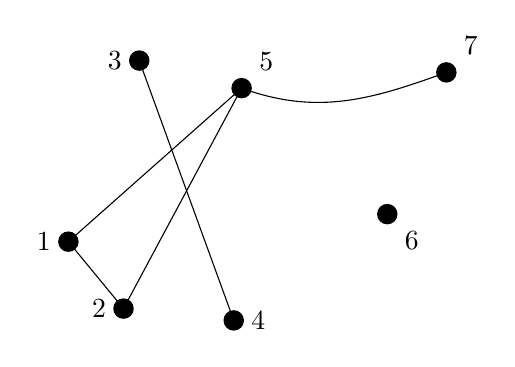
\begin{tikzpicture}[>=latex]
	\coordinate (C) at (-1.6,1.55);
	\coordinate (D) at (-0.4,-1.75);
	\coordinate (B) at (-1.8,-1.6);
	\coordinate (A) at (-2.5,-0.75);
	\coordinate (E) at (-0.3,1.2);
	\coordinate (F) at (1.55,-0.4);
	\coordinate (G) at (2.3,1.4);
	\fill (C) circle  (3.7pt)  node  [left=1mm]   {\(3\)};
	\fill (D) circle  (3.7pt)  node  [right=1mm]  {\(4\)};
	\fill (B) circle  (3.7pt)  node  [left=1mm]   {\(2\)};
	\fill (A) circle  (3.7pt)  node  [left=1mm]   {\(1\)};
	\fill (E) circle  (3.7pt)  node  [above   right=1mm]    {\(5\)};
	\fill (F) circle  (3.7pt)  node  [below   right=1mm]    {\(6\)};
	\fill (G) circle  (3.7pt)  node  [above   right=1mm]    {\(7\)};
	\draw (A) -- (E) -- (B) -- cycle;
	\draw (C) -- (D);
	\draw (E) to [out=-20 , in=200] (G);
\end{tikzpicture}

\end{document}
